% Options for packages loaded elsewhere
\PassOptionsToPackage{unicode}{hyperref}
\PassOptionsToPackage{hyphens}{url}
%
\documentclass[
]{book}
\usepackage{amsmath,amssymb}
\usepackage{lmodern}
\usepackage{iftex}
\ifPDFTeX
  \usepackage[T1]{fontenc}
  \usepackage[utf8]{inputenc}
  \usepackage{textcomp} % provide euro and other symbols
\else % if luatex or xetex
  \usepackage{unicode-math}
  \defaultfontfeatures{Scale=MatchLowercase}
  \defaultfontfeatures[\rmfamily]{Ligatures=TeX,Scale=1}
\fi
% Use upquote if available, for straight quotes in verbatim environments
\IfFileExists{upquote.sty}{\usepackage{upquote}}{}
\IfFileExists{microtype.sty}{% use microtype if available
  \usepackage[]{microtype}
  \UseMicrotypeSet[protrusion]{basicmath} % disable protrusion for tt fonts
}{}
\makeatletter
\@ifundefined{KOMAClassName}{% if non-KOMA class
  \IfFileExists{parskip.sty}{%
    \usepackage{parskip}
  }{% else
    \setlength{\parindent}{0pt}
    \setlength{\parskip}{6pt plus 2pt minus 1pt}}
}{% if KOMA class
  \KOMAoptions{parskip=half}}
\makeatother
\usepackage{xcolor}
\usepackage{color}
\usepackage{fancyvrb}
\newcommand{\VerbBar}{|}
\newcommand{\VERB}{\Verb[commandchars=\\\{\}]}
\DefineVerbatimEnvironment{Highlighting}{Verbatim}{commandchars=\\\{\}}
% Add ',fontsize=\small' for more characters per line
\usepackage{framed}
\definecolor{shadecolor}{RGB}{248,248,248}
\newenvironment{Shaded}{\begin{snugshade}}{\end{snugshade}}
\newcommand{\AlertTok}[1]{\textcolor[rgb]{0.94,0.16,0.16}{#1}}
\newcommand{\AnnotationTok}[1]{\textcolor[rgb]{0.56,0.35,0.01}{\textbf{\textit{#1}}}}
\newcommand{\AttributeTok}[1]{\textcolor[rgb]{0.77,0.63,0.00}{#1}}
\newcommand{\BaseNTok}[1]{\textcolor[rgb]{0.00,0.00,0.81}{#1}}
\newcommand{\BuiltInTok}[1]{#1}
\newcommand{\CharTok}[1]{\textcolor[rgb]{0.31,0.60,0.02}{#1}}
\newcommand{\CommentTok}[1]{\textcolor[rgb]{0.56,0.35,0.01}{\textit{#1}}}
\newcommand{\CommentVarTok}[1]{\textcolor[rgb]{0.56,0.35,0.01}{\textbf{\textit{#1}}}}
\newcommand{\ConstantTok}[1]{\textcolor[rgb]{0.00,0.00,0.00}{#1}}
\newcommand{\ControlFlowTok}[1]{\textcolor[rgb]{0.13,0.29,0.53}{\textbf{#1}}}
\newcommand{\DataTypeTok}[1]{\textcolor[rgb]{0.13,0.29,0.53}{#1}}
\newcommand{\DecValTok}[1]{\textcolor[rgb]{0.00,0.00,0.81}{#1}}
\newcommand{\DocumentationTok}[1]{\textcolor[rgb]{0.56,0.35,0.01}{\textbf{\textit{#1}}}}
\newcommand{\ErrorTok}[1]{\textcolor[rgb]{0.64,0.00,0.00}{\textbf{#1}}}
\newcommand{\ExtensionTok}[1]{#1}
\newcommand{\FloatTok}[1]{\textcolor[rgb]{0.00,0.00,0.81}{#1}}
\newcommand{\FunctionTok}[1]{\textcolor[rgb]{0.00,0.00,0.00}{#1}}
\newcommand{\ImportTok}[1]{#1}
\newcommand{\InformationTok}[1]{\textcolor[rgb]{0.56,0.35,0.01}{\textbf{\textit{#1}}}}
\newcommand{\KeywordTok}[1]{\textcolor[rgb]{0.13,0.29,0.53}{\textbf{#1}}}
\newcommand{\NormalTok}[1]{#1}
\newcommand{\OperatorTok}[1]{\textcolor[rgb]{0.81,0.36,0.00}{\textbf{#1}}}
\newcommand{\OtherTok}[1]{\textcolor[rgb]{0.56,0.35,0.01}{#1}}
\newcommand{\PreprocessorTok}[1]{\textcolor[rgb]{0.56,0.35,0.01}{\textit{#1}}}
\newcommand{\RegionMarkerTok}[1]{#1}
\newcommand{\SpecialCharTok}[1]{\textcolor[rgb]{0.00,0.00,0.00}{#1}}
\newcommand{\SpecialStringTok}[1]{\textcolor[rgb]{0.31,0.60,0.02}{#1}}
\newcommand{\StringTok}[1]{\textcolor[rgb]{0.31,0.60,0.02}{#1}}
\newcommand{\VariableTok}[1]{\textcolor[rgb]{0.00,0.00,0.00}{#1}}
\newcommand{\VerbatimStringTok}[1]{\textcolor[rgb]{0.31,0.60,0.02}{#1}}
\newcommand{\WarningTok}[1]{\textcolor[rgb]{0.56,0.35,0.01}{\textbf{\textit{#1}}}}
\usepackage{longtable,booktabs,array}
\usepackage{calc} % for calculating minipage widths
% Correct order of tables after \paragraph or \subparagraph
\usepackage{etoolbox}
\makeatletter
\patchcmd\longtable{\par}{\if@noskipsec\mbox{}\fi\par}{}{}
\makeatother
% Allow footnotes in longtable head/foot
\IfFileExists{footnotehyper.sty}{\usepackage{footnotehyper}}{\usepackage{footnote}}
\makesavenoteenv{longtable}
\usepackage{graphicx}
\makeatletter
\def\maxwidth{\ifdim\Gin@nat@width>\linewidth\linewidth\else\Gin@nat@width\fi}
\def\maxheight{\ifdim\Gin@nat@height>\textheight\textheight\else\Gin@nat@height\fi}
\makeatother
% Scale images if necessary, so that they will not overflow the page
% margins by default, and it is still possible to overwrite the defaults
% using explicit options in \includegraphics[width, height, ...]{}
\setkeys{Gin}{width=\maxwidth,height=\maxheight,keepaspectratio}
% Set default figure placement to htbp
\makeatletter
\def\fps@figure{htbp}
\makeatother
\setlength{\emergencystretch}{3em} % prevent overfull lines
\providecommand{\tightlist}{%
  \setlength{\itemsep}{0pt}\setlength{\parskip}{0pt}}
\setcounter{secnumdepth}{5}
\usepackage{booktabs}
\usepackage{longtable}
\usepackage{array}
\usepackage{multirow}
\usepackage{wrapfig}
\usepackage{float}
\usepackage{colortbl}
\usepackage{pdflscape}
\usepackage{tabu}
\usepackage{threeparttable}
\usepackage{threeparttablex}
\usepackage[normalem]{ulem}
\usepackage{makecell}
\usepackage{xcolor}
\ifLuaTeX
  \usepackage{selnolig}  % disable illegal ligatures
\fi
\usepackage[]{natbib}
\bibliographystyle{apalike}
\IfFileExists{bookmark.sty}{\usepackage{bookmark}}{\usepackage{hyperref}}
\IfFileExists{xurl.sty}{\usepackage{xurl}}{} % add URL line breaks if available
\urlstyle{same} % disable monospaced font for URLs
\hypersetup{
  pdftitle={MODELOS SEMI ESTRUCTURALES PARA EL CRÉDITO AL CONSUMO},
  pdfauthor={Luis Ortiz-Cevallos},
  hidelinks,
  pdfcreator={LaTeX via pandoc}}

\title{MODELOS SEMI ESTRUCTURALES PARA EL CRÉDITO AL CONSUMO}
\author{\href{https://ortiz-cevallos.github.io/MYSELF/}{Luis Ortiz-Cevallos}}
\date{2023-03-31}

\begin{document}
\maketitle

{
\setcounter{tocdepth}{1}
\tableofcontents
}
\hypertarget{aplicaciuxf3n-para-guatemala}{%
\chapter{Aplicación para Guatemala}\label{aplicaciuxf3n-para-guatemala}}

\hypertarget{blanchard-quah-ortogonalizaciuxf3n-restricciones-sobre-c1}{%
\section{Blanchard-Quah ortogonalización (restricciones) sobre C(1)}\label{blanchard-quah-ortogonalizaciuxf3n-restricciones-sobre-c1}}

Al observar la evolución del crédito hacia consumo provisto por el sistema bancario guatemalteco y disponible en \citet{SECMCADATOS}, se observa una series con una tendendencia estocástica.

\begin{Shaded}
\begin{Highlighting}[]
\FunctionTok{library}\NormalTok{(}\StringTok{"zoo"}\NormalTok{)}
\FunctionTok{library}\NormalTok{(}\StringTok{"xts"}\NormalTok{)}
\FunctionTok{library}\NormalTok{(dplyr)}
\FunctionTok{library}\NormalTok{(ggplot2)}
\FunctionTok{library}\NormalTok{(kableExtra)}
\FunctionTok{library}\NormalTok{(xtable)}
\FunctionTok{library}\NormalTok{(tidyr)}
\FunctionTok{library}\NormalTok{(quantmod)}
\FunctionTok{library}\NormalTok{(RColorBrewer)}
\FunctionTok{library}\NormalTok{(gridExtra)}
\CommentTok{\#CARGAMOS DATOS MENSUALES}
\NormalTok{DATA\_MES}\OtherTok{\textless{}{-}}\FunctionTok{as.xts}\NormalTok{(}\FunctionTok{read.zoo}\NormalTok{(}\StringTok{"GT\_MES.csv"}\NormalTok{, }\AttributeTok{index.column =} \DecValTok{1}\NormalTok{,}
          \AttributeTok{sep =} \StringTok{";"}\NormalTok{, }\AttributeTok{header=}\ConstantTok{TRUE}\NormalTok{, }\AttributeTok{format =} \StringTok{"\%Y{-}\%m{-}\%d"}\NormalTok{))}
\NormalTok{CREDITO}\OtherTok{\textless{}{-}}\NormalTok{DATA\_MES}\SpecialCharTok{$}\NormalTok{CRED}
\NormalTok{CREDITO}\OtherTok{\textless{}{-}}\FunctionTok{data.frame}\NormalTok{(}\AttributeTok{date=}\FunctionTok{index}\NormalTok{(CREDITO), }\FunctionTok{coredata}\NormalTok{(CREDITO))}
\NormalTok{CREDITO}\OtherTok{\textless{}{-}}\FunctionTok{filter}\NormalTok{(CREDITO, date }\SpecialCharTok{\textgreater{}=} \StringTok{"2008{-}01{-}01"}\NormalTok{)}
\FunctionTok{colnames}\NormalTok{(CREDITO)}\OtherTok{\textless{}{-}}\FunctionTok{c}\NormalTok{(}\StringTok{"date"}\NormalTok{,}\StringTok{"CREDITO"}\NormalTok{)}
\NormalTok{CREDITO}\OtherTok{\textless{}{-}}\FunctionTok{mutate}\NormalTok{(CREDITO, }\AttributeTok{CONSUMO=}\FunctionTok{log}\NormalTok{(CREDITO))}
\NormalTok{G}\OtherTok{\textless{}{-}}\FunctionTok{ggplot}\NormalTok{(CREDITO, }\FunctionTok{aes}\NormalTok{(}\AttributeTok{x=}\NormalTok{date, }\AttributeTok{y=}\NormalTok{CONSUMO))}
\NormalTok{G}\OtherTok{\textless{}{-}}\NormalTok{G}\SpecialCharTok{+}\FunctionTok{labs}\NormalTok{(}\AttributeTok{y=}\StringTok{"Logaritmo"}\NormalTok{,}
          \AttributeTok{x=}\StringTok{"Fecha"}\NormalTok{, }\AttributeTok{title =} \StringTok{"Guatemala: evolución del crédito al consumo"}\NormalTok{,}
          \AttributeTok{caption =} \StringTok{"https://www.secmca.org/wp{-}content/uploads/2023/03/REPORTE\_INDICADO}
\StringTok{RES\_BANCARIOS\_MARZO\_2023.xlsx"}\NormalTok{)}\SpecialCharTok{+}
  \FunctionTok{geom\_line}\NormalTok{(}\AttributeTok{size=}\FloatTok{1.5}\NormalTok{)}
\NormalTok{G}
\end{Highlighting}
\end{Shaded}

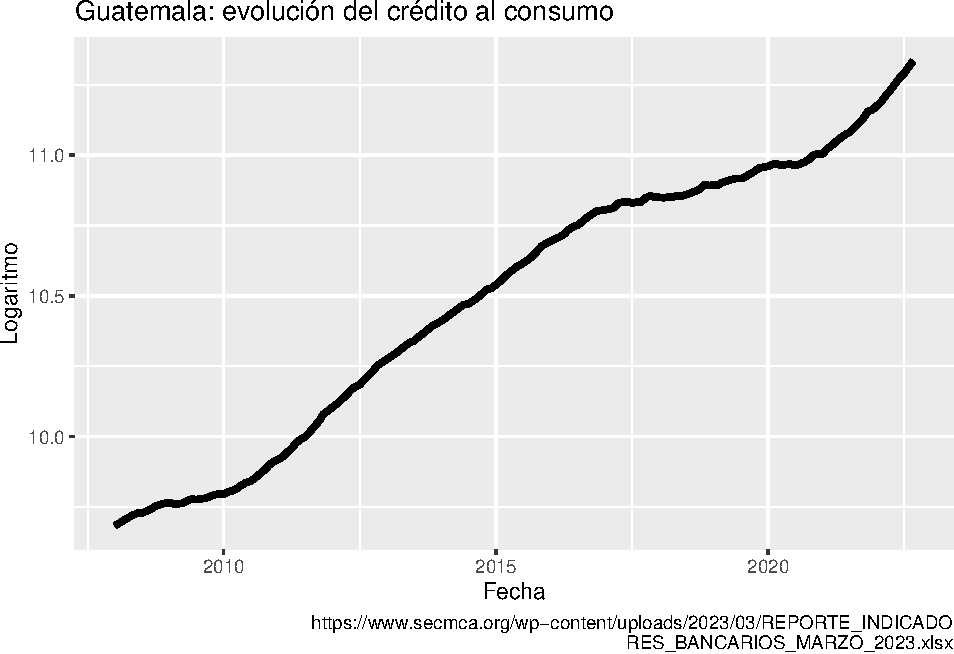
\includegraphics{01-conceptos_files/figure-latex/unnamed-chunk-1-1.pdf}

El proceso de generación de la serie del crédito al consumo puede explicarse a través de la identificación de diferentes innovaciones. Una de ellas, las llamaré tecnológicas (en general uso ese término para referir los factores que pueden producir una mayor inclusión financiera independientemente si es producto de políticas o nuevas tecnologías), la segunda las de denanda y la tercera de absorción fiscal.

Para este ejercicio de identificación sigo la metodología propuesta por \citet{BLANCHARD88} y estimo la forma reducida de un Vector Autorregresivo integrado por la tasa de crecimiento de la cartera de consumo nominal (\(\Delta c_{t}\)), la tasa de crecimiento del PIB (\(\Delta y_{t}\)) y el porcentaje de los activos de los sistemas bancarios en títulos y valores públicos (\(\Delta y_{t}\)). La representación de este VAR como un proceso de media móviles está dado por:

\begin{equation}
X_{t}=\left( \begin{array}{c}
\Delta c_{t} \\
\Delta y_{t} \\
\Delta x_{t} 
\end{array}
\right)=A(L)e_{t}
\label{e1}
\end{equation}

Considero \(A(0)=I\) y \(\Sigma_e=E(e e^{\tau})\) como la matriz de varianza y covarianza de la forma reducida del VAR mostrado en \ref{e1}. Y supongo, primero que el crédito hacia consumo, la actividad económica y la exposición del sistema bancario hacia valores del gobierno son producidos a través de tres procesos estructurales independientes con shocks de varianza unitaria. Y segundo, que uno de esos procesos, el de las innovaciones tecnológicas, es el responsable de la tendencia estocástica observada en el crédito para consumo. Con base en lo anterior defino un VAR estructural cuya representación como un proceso de medias móviles es el siguiente:

\begin{equation}
X_{t}=C(L)\epsilon_{t}=\left( \begin{array}{ccc}
C_{1,1}(L) & C_{1,2}(L) & C_{1,3}(L)\\
C_{2,1}(L) & C_{2,2}(L) & C_{2,3}(L)\\
C_{3,1}(L) & C_{3,2}(L) & C_{3,3}(L)
\end{array}
\right)\epsilon_{t}
\label{e2}
\end{equation}

Siendo \(\Sigma_{\epsilon}=E(\epsilon \epsilon^{\tau})=I\) la matriz de varianza y covarianza de los shocks estructurales, los cuales son independientes y con varianza unitaria, y \(C_{1,2}(1)=C_{1,3}(1)=0\), indicando que el shock de demanda y fiscal sobre las variables tasa de crecimiento del PIB y porcentaje de activos invertidos en valores soberanos, en su orden, no tienen efectos de largo plazo en el crédito nominal para consumo.

El proceso y resultado de la estimación es el siguiente:

\begin{Shaded}
\begin{Highlighting}[]
\NormalTok{CRED       }\OtherTok{\textless{}{-}}\NormalTok{DATA\_MES}\SpecialCharTok{$}\NormalTok{CRED}
\NormalTok{FISCAL     }\OtherTok{\textless{}{-}}\NormalTok{DATA\_MES}\SpecialCharTok{$}\NormalTok{PUB}
\NormalTok{CRED       }\OtherTok{\textless{}{-}}\NormalTok{CRED[}\StringTok{"2008{-}01{-}01/2022{-}09{-}01"}\NormalTok{]}
\NormalTok{ep1        }\OtherTok{\textless{}{-}}\FunctionTok{endpoints}\NormalTok{(CRED , }\AttributeTok{on =} \StringTok{"quarters"}\NormalTok{)}
\NormalTok{CRED       }\OtherTok{\textless{}{-}}\FunctionTok{period.apply}\NormalTok{(CRED  , }\AttributeTok{INDEX =}\NormalTok{ ep1, }\AttributeTok{FUN =}\NormalTok{ sum)}
\NormalTok{DCRED      }\OtherTok{\textless{}{-}}\FunctionTok{diff}\NormalTok{(}\DecValTok{100}\SpecialCharTok{*}\FunctionTok{log}\NormalTok{(CRED ), }\AttributeTok{lag=}\DecValTok{4}\NormalTok{)}
\NormalTok{FISCAL     }\OtherTok{\textless{}{-}}\NormalTok{FISCAL[}\StringTok{"2008{-}01{-}01/2022{-}09{-}01"}\NormalTok{]}
\NormalTok{ep2        }\OtherTok{\textless{}{-}}\FunctionTok{endpoints}\NormalTok{(FISCAL , }\AttributeTok{on =} \StringTok{"quarters"}\NormalTok{)}
\NormalTok{TASA       }\OtherTok{\textless{}{-}}\FunctionTok{period.apply}\NormalTok{(FISCAL, }\AttributeTok{INDEX =}\NormalTok{ ep2, }\AttributeTok{FUN =}\NormalTok{ max)}
\NormalTok{DATA\_TRIM   }\OtherTok{\textless{}{-}}\FunctionTok{as.xts}\NormalTok{(}\FunctionTok{read.zoo}\NormalTok{(}\StringTok{"TRIM\_GT.csv"}\NormalTok{, }\AttributeTok{index.column =} \DecValTok{1}\NormalTok{,}
                      \AttributeTok{sep =} \StringTok{";"}\NormalTok{, }\AttributeTok{header=}\ConstantTok{TRUE}\NormalTok{, }\AttributeTok{format =} \StringTok{"\%Y{-}\%m{-}\%d"}\NormalTok{))}
\NormalTok{PIB         }\OtherTok{\textless{}{-}}\NormalTok{DATA\_TRIM}\SpecialCharTok{$}\NormalTok{PIB}
\NormalTok{PIB         }\OtherTok{\textless{}{-}}\NormalTok{PIB[}\StringTok{"2001{-}03{-}01/2022{-}09{-}01"}\NormalTok{]}
\NormalTok{DPIB        }\OtherTok{\textless{}{-}}\FunctionTok{diff}\NormalTok{(}\DecValTok{100}\SpecialCharTok{*}\FunctionTok{log}\NormalTok{(PIB), }\AttributeTok{lag=}\DecValTok{4}\NormalTok{)}
\CommentTok{\#COMBINAR}
\NormalTok{BASE       }\OtherTok{\textless{}{-}}\FunctionTok{merge}\NormalTok{(DCRED, DPIB,}\AttributeTok{join=}\StringTok{"left"}\NormalTok{)}
\NormalTok{BASE       }\OtherTok{\textless{}{-}}\FunctionTok{merge}\NormalTok{(BASE,  FISCAL,}\AttributeTok{join=}\StringTok{"left"}\NormalTok{)}
\NormalTok{BASE       }\OtherTok{\textless{}{-}}\FunctionTok{data.frame}\NormalTok{(}\AttributeTok{date=}\FunctionTok{index}\NormalTok{(BASE), }\FunctionTok{coredata}\NormalTok{(BASE))}
\FunctionTok{colnames}\NormalTok{(BASE)}\OtherTok{\textless{}{-}}\FunctionTok{c}\NormalTok{(}\StringTok{"date"}\NormalTok{,}\StringTok{"c"}\NormalTok{, }\StringTok{"y"}\NormalTok{, }\StringTok{\textquotesingle{}x\textquotesingle{}}\NormalTok{)}
\NormalTok{DATA       }\OtherTok{\textless{}{-}}\NormalTok{dplyr}\SpecialCharTok{::}\FunctionTok{select}\NormalTok{(BASE, date, c,y,x)}
\FunctionTok{colnames}\NormalTok{(DATA)}\OtherTok{\textless{}{-}}\FunctionTok{c}\NormalTok{(}\StringTok{"date"}\NormalTok{, }\StringTok{"c"}\NormalTok{, }\StringTok{"y"}\NormalTok{, }\StringTok{\textquotesingle{}x\textquotesingle{}}\NormalTok{)}
\NormalTok{DATA       }\OtherTok{\textless{}{-}}\FunctionTok{filter}\NormalTok{(DATA, date }\SpecialCharTok{\textgreater{}=} \StringTok{"2016{-}03{-}01"}\NormalTok{)}
\NormalTok{DATA       }\OtherTok{\textless{}{-}}\FunctionTok{xts}\NormalTok{(DATA[,}\SpecialCharTok{{-}}\DecValTok{1}\NormalTok{], }\AttributeTok{order.by=}\FunctionTok{as.Date}\NormalTok{(DATA[,}\DecValTok{1}\NormalTok{], }\StringTok{"\%Y/\%m/\%d"}\NormalTok{))}
\FunctionTok{library}\NormalTok{(}\StringTok{"svars"}\NormalTok{)}
\NormalTok{VAR        }\OtherTok{\textless{}{-}}\NormalTok{ vars}\SpecialCharTok{::}\FunctionTok{VAR}\NormalTok{(DATA[,}\FunctionTok{c}\NormalTok{(}\DecValTok{1}\NormalTok{,}\DecValTok{2}\NormalTok{,}\DecValTok{3}\NormalTok{)],}\AttributeTok{p =}\DecValTok{2}\NormalTok{,}\AttributeTok{type =} \StringTok{"const"}\NormalTok{)}
\NormalTok{VAR}\SpecialCharTok{$}\NormalTok{varresult}\SpecialCharTok{$}\NormalTok{c}\SpecialCharTok{$}\NormalTok{coefficients}
\end{Highlighting}
\end{Shaded}

\begin{verbatim}
##        c.l1        y.l1        x.l1        c.l2        y.l2        x.l2 
##  1.12127681  0.15372782  0.29159136 -0.11201301 -0.01109658  0.18036079 
##       const 
## -9.91395632
\end{verbatim}

\begin{Shaded}
\begin{Highlighting}[]
\NormalTok{VAR}\SpecialCharTok{$}\NormalTok{varresult}\SpecialCharTok{$}\NormalTok{y}\SpecialCharTok{$}\NormalTok{coefficients}
\end{Highlighting}
\end{Shaded}

\begin{verbatim}
##        c.l1        y.l1        x.l1        c.l2        y.l2        x.l2 
## -0.25412909  0.57678412  0.39960337  0.27004423 -0.15357170 -0.02784201 
##       const 
## -5.84527946
\end{verbatim}

\begin{Shaded}
\begin{Highlighting}[]
\NormalTok{VAR}\SpecialCharTok{$}\NormalTok{varresult}\SpecialCharTok{$}\NormalTok{x}\SpecialCharTok{$}\NormalTok{coefficients}
\end{Highlighting}
\end{Shaded}

\begin{verbatim}
##        c.l1        y.l1        x.l1        c.l2        y.l2        x.l2 
##  0.18016081 -0.13225215  0.28849915 -0.26998876 -0.03531496  0.45762387 
##       const 
##  6.70493277
\end{verbatim}

\begin{Shaded}
\begin{Highlighting}[]
\NormalTok{SIGMA}\OtherTok{\textless{}{-}}\FunctionTok{summary}\NormalTok{(VAR)}
\NormalTok{SIGMA}\SpecialCharTok{$}\NormalTok{covres}
\end{Highlighting}
\end{Shaded}

\begin{verbatim}
##           c         y         x
## c 1.2422579  2.067672 0.1369263
## y 2.0676722 13.450295 0.5679060
## x 0.1369263  0.567906 1.6557099
\end{verbatim}

Habiendo estimado el VAR a continuación encontramos las restricciones de corto o contemporáneas y largo plazo:

\begin{Shaded}
\begin{Highlighting}[]
\NormalTok{BQMODEL}\OtherTok{\textless{}{-}} \FunctionTok{BQ}\NormalTok{(VAR)}
\FunctionTok{summary}\NormalTok{(BQMODEL)}
\end{Highlighting}
\end{Shaded}

\begin{verbatim}
## 
## SVAR Estimation Results:
## ======================== 
## 
## Call:
## BQ(x = VAR)
## 
## Type: Blanchard-Quah 
## Sample size: 25 
## Log Likelihood: -144.025 
## 
## Estimated contemporaneous impact matrix:
##         c      y       x
## c 0.45904 0.3686 -0.9464
## y 0.08455 3.5899 -0.7455
## x 1.15782 0.2366  0.5091
## 
## Estimated identified long run impact matrix:
##         c      y     x
## c 16.7627  0.000 0.000
## y -0.1924  4.788 0.000
## x -1.2435 -2.228 2.005
## 
## Covariance matrix of reduced form residuals (*100):
##        c       y      x
## c 124.23  206.77  13.69
## y 206.77 1345.03  56.79
## x  13.69   56.79 165.57
\end{verbatim}

En seguida, calculamos la función impulso respuesta para cada variable, teniendo en cuenta que el PIB y la proporción de activos del sistema bancario invertidos en títulos y valores del gobierno no sufren en el largo plazo ningún efecto de los tres shocks estructurales.

\begin{Shaded}
\begin{Highlighting}[]
\NormalTok{FIR\_BQ }\OtherTok{\textless{}{-}} \FunctionTok{irf}\NormalTok{(BQMODEL,}\AttributeTok{n.ahead =} \DecValTok{32}\NormalTok{, }\AttributeTok{impulse =} \FunctionTok{c}\NormalTok{( }\StringTok{"c"}\NormalTok{, }\StringTok{"y"}\NormalTok{, }\StringTok{"x"}\NormalTok{), }\AttributeTok{boot =}\ConstantTok{FALSE}\NormalTok{)}
\NormalTok{tecno  }\OtherTok{\textless{}{-}} \FunctionTok{cbind}\NormalTok{(}\FunctionTok{cumsum}\NormalTok{(FIR\_BQ}\SpecialCharTok{$}\NormalTok{irf}\SpecialCharTok{$}\NormalTok{c[, }\DecValTok{1}\NormalTok{]), FIR\_BQ}\SpecialCharTok{$}\NormalTok{irf}\SpecialCharTok{$}\NormalTok{c[, }\DecValTok{2}\NormalTok{],  FIR\_BQ}\SpecialCharTok{$}\NormalTok{irf}\SpecialCharTok{$}\NormalTok{c[, }\DecValTok{3}\NormalTok{])}
\NormalTok{RESULTADO1}\OtherTok{\textless{}{-}}\FunctionTok{as.data.frame}\NormalTok{(tecno)}
\NormalTok{PERIODO}\OtherTok{\textless{}{-}}\FunctionTok{seq}\NormalTok{(}\DecValTok{1}\NormalTok{,}\DecValTok{33}\NormalTok{,}\DecValTok{1}\NormalTok{)}
\NormalTok{RESULTADO1 }\OtherTok{\textless{}{-}}\FunctionTok{cbind}\NormalTok{(RESULTADO1,PERIODO)}
\NormalTok{CODE}\OtherTok{\textless{}{-}}\FunctionTok{rep}\NormalTok{(}\StringTok{"Tecnológico"}\NormalTok{,}\DecValTok{33}\NormalTok{)}
\NormalTok{RESULTADO1 }\OtherTok{\textless{}{-}}\FunctionTok{cbind}\NormalTok{(RESULTADO1,CODE)}
\DocumentationTok{\#\#\#\#\#\#\#\#\#\#\#\#\#\#\#\#\#\#\#\#\#\#\#\#\#\#\#\#\#\#\#\#\#\#\#\#\#\#}
\NormalTok{demanda }\OtherTok{\textless{}{-}} \FunctionTok{cbind}\NormalTok{(FIR\_BQ}\SpecialCharTok{$}\NormalTok{irf}\SpecialCharTok{$}\NormalTok{y[, }\DecValTok{1}\NormalTok{], FIR\_BQ}\SpecialCharTok{$}\NormalTok{irf}\SpecialCharTok{$}\NormalTok{y[, }\DecValTok{2}\NormalTok{],  FIR\_BQ}\SpecialCharTok{$}\NormalTok{irf}\SpecialCharTok{$}\NormalTok{y[, }\DecValTok{3}\NormalTok{])}
\NormalTok{RESULTADO2}\OtherTok{\textless{}{-}}\FunctionTok{as.data.frame}\NormalTok{(demanda)}
\NormalTok{RESULTADO2 }\OtherTok{\textless{}{-}}\FunctionTok{cbind}\NormalTok{(RESULTADO2,PERIODO)}
\NormalTok{CODE}\OtherTok{\textless{}{-}}\FunctionTok{rep}\NormalTok{(}\StringTok{"Demanda"}\NormalTok{,}\DecValTok{33}\NormalTok{)}
\NormalTok{RESULTADO2 }\OtherTok{\textless{}{-}}\FunctionTok{cbind}\NormalTok{(RESULTADO2,CODE)}
\DocumentationTok{\#\#\#\#\#\#\#\#\#\#\#\#\#\#\#\#\#\#\#\#\#\#\#\#\#\#\#\#\#\#\#\#\#\#\#\#\#\#}
\NormalTok{fiscal }\OtherTok{\textless{}{-}} \FunctionTok{cbind}\NormalTok{(}\SpecialCharTok{{-}}\DecValTok{1}\SpecialCharTok{*}\NormalTok{FIR\_BQ}\SpecialCharTok{$}\NormalTok{irf}\SpecialCharTok{$}\NormalTok{x[, }\DecValTok{1}\NormalTok{], }\SpecialCharTok{{-}}\DecValTok{1}\SpecialCharTok{*}\NormalTok{FIR\_BQ}\SpecialCharTok{$}\NormalTok{irf}\SpecialCharTok{$}\NormalTok{x[, }\DecValTok{2}\NormalTok{], }\SpecialCharTok{{-}}\DecValTok{1}\SpecialCharTok{*}\NormalTok{FIR\_BQ}\SpecialCharTok{$}\NormalTok{irf}\SpecialCharTok{$}\NormalTok{x[, }\DecValTok{3}\NormalTok{])}
\NormalTok{RESULTADO3 }\OtherTok{\textless{}{-}}\FunctionTok{as.data.frame}\NormalTok{(fiscal)}
\NormalTok{RESULTADO3 }\OtherTok{\textless{}{-}}\FunctionTok{cbind}\NormalTok{(RESULTADO3,PERIODO)}
\NormalTok{CODE}\OtherTok{\textless{}{-}}\FunctionTok{rep}\NormalTok{(}\StringTok{"Fiscal"}\NormalTok{,}\DecValTok{33}\NormalTok{)}
\NormalTok{RESULTADO3}\OtherTok{\textless{}{-}}\FunctionTok{cbind}\NormalTok{(RESULTADO3,CODE)}
\NormalTok{RESULTADO }\OtherTok{\textless{}{-}}\FunctionTok{rbind}\NormalTok{(RESULTADO1,RESULTADO2,RESULTADO3)}
\NormalTok{BASE\_LONG }\OtherTok{\textless{}{-}} \FunctionTok{gather}\NormalTok{(RESULTADO, }\AttributeTok{key=}\StringTok{"measure"}\NormalTok{, }\AttributeTok{value=}\StringTok{"value"}\NormalTok{,}\FunctionTok{c}\NormalTok{(}\StringTok{"V1"}\NormalTok{, }\StringTok{"V2"}\NormalTok{, }\StringTok{"V3"}\NormalTok{))}
\NormalTok{BASE\_LONG}\SpecialCharTok{$}\NormalTok{measure }\OtherTok{\textless{}{-}} \FunctionTok{factor}\NormalTok{(BASE\_LONG}\SpecialCharTok{$}\NormalTok{measure,}\AttributeTok{levels =}\NormalTok{ ,}\FunctionTok{c}\NormalTok{(}\StringTok{"V1"}\NormalTok{, }\StringTok{"V2"}\NormalTok{, }\StringTok{"V3"}\NormalTok{))}
\NormalTok{BASE\_LONG}\SpecialCharTok{$}\NormalTok{CODE }\OtherTok{\textless{}{-}} \FunctionTok{factor}\NormalTok{(BASE\_LONG}\SpecialCharTok{$}\NormalTok{CODE,}\AttributeTok{levels =} \FunctionTok{c}\NormalTok{(}\StringTok{"Tecnológico"}\NormalTok{, }\StringTok{"Demanda"}\NormalTok{, }\StringTok{"Fiscal"}\NormalTok{))}

\NormalTok{variable\_names }\OtherTok{\textless{}{-}} \FunctionTok{list}\NormalTok{(}
  \StringTok{"Tecnológico"} \OtherTok{=} \StringTok{"Shock tecnológicos"}\NormalTok{, }
  \StringTok{"Demanda"} \OtherTok{=} \StringTok{"Shock de demanda"}\NormalTok{,}
  \StringTok{"Fiscal"} \OtherTok{=} \StringTok{"Shock fiscal"}
\NormalTok{)}

\NormalTok{variable\_labeller2 }\OtherTok{\textless{}{-}} \ControlFlowTok{function}\NormalTok{(variable,value)\{}
  \ControlFlowTok{if}\NormalTok{ (variable}\SpecialCharTok{==}\StringTok{\textquotesingle{}CODE\textquotesingle{}}\NormalTok{) \{}
    \FunctionTok{return}\NormalTok{(variable\_names[value])}
\NormalTok{  \} }\ControlFlowTok{else}\NormalTok{ \{}
    \FunctionTok{return}\NormalTok{(region\_names)}
\NormalTok{  \}}
\NormalTok{\}}
\NormalTok{paleta}\OtherTok{\textless{}{-}}\FunctionTok{c}\NormalTok{(}\StringTok{"blue"}\NormalTok{,}\StringTok{"red"}\NormalTok{, }\StringTok{"burlywood"}\NormalTok{)}
\NormalTok{Z}\OtherTok{\textless{}{-}}\FunctionTok{ggplot}\NormalTok{(BASE\_LONG, }\FunctionTok{aes}\NormalTok{(}\AttributeTok{x=}\NormalTok{PERIODO, }\AttributeTok{y=}\NormalTok{value, }\AttributeTok{group =}\NormalTok{ measure,}
                         \AttributeTok{colour=}\NormalTok{measure))}\SpecialCharTok{+}
  \FunctionTok{facet\_wrap}\NormalTok{(.}\SpecialCharTok{\textasciitilde{}}\NormalTok{CODE, }\AttributeTok{scales=}\StringTok{"free"}\NormalTok{, }\AttributeTok{labeller=}\NormalTok{ variable\_labeller2)}
\NormalTok{Z}\OtherTok{\textless{}{-}}\NormalTok{Z}\SpecialCharTok{+}\FunctionTok{labs}\NormalTok{(}\AttributeTok{y=}\StringTok{"Respuesta (\%)"}\NormalTok{,}
          \AttributeTok{x=}\StringTok{"Períodos (trimestres)"}\NormalTok{, }\AttributeTok{title =} \StringTok{"Guatemala: funciones impulso respuestas"}\NormalTok{,}
          \AttributeTok{caption =} \StringTok{"Elaboración propia con base en: https://www.secmca.org/wp{-}content/uploads/2023/03/REPORTE\_INDICADO}
\StringTok{RES\_BANCARIOS\_MARZO\_2023.xlsx"}\NormalTok{)}\SpecialCharTok{+}
  \FunctionTok{geom\_hline}\NormalTok{(}\AttributeTok{yintercept=}\DecValTok{0}\NormalTok{, }\AttributeTok{linetype=}\StringTok{"dashed"}\NormalTok{,}
             \AttributeTok{color =} \StringTok{"black"}\NormalTok{, }\AttributeTok{size=}\DecValTok{1}\NormalTok{)}\SpecialCharTok{+}
  \FunctionTok{geom\_line}\NormalTok{(}\AttributeTok{size=}\FloatTok{1.5}\NormalTok{)}\SpecialCharTok{+}
  \FunctionTok{scale\_color\_manual}\NormalTok{(}\AttributeTok{values=}\NormalTok{paleta,}
                     \AttributeTok{labels =} \FunctionTok{c}\NormalTok{(}\StringTok{"Crédito para consumo"}\NormalTok{,}
                                \StringTok{"Producto"}\NormalTok{,}
                                \StringTok{"Proporción de los activos invertidos en valores públicos"}
\NormalTok{                                ))}
\NormalTok{Z}\OtherTok{\textless{}{-}}\NormalTok{Z}\SpecialCharTok{+}\FunctionTok{theme}\NormalTok{(}\AttributeTok{axis.line.x =} \FunctionTok{element\_line}\NormalTok{(}\AttributeTok{colour =} \StringTok{"black"}\NormalTok{, }\AttributeTok{size =} \FloatTok{0.5}\NormalTok{),}
           \AttributeTok{axis.line.y.left  =} \FunctionTok{element\_line}\NormalTok{(}\AttributeTok{colour =} \StringTok{"black"}\NormalTok{, }\AttributeTok{size =} \FloatTok{0.5}\NormalTok{),}
           \AttributeTok{axis.line.y.right =} \FunctionTok{element\_blank}\NormalTok{(),}
           \AttributeTok{axis.text.x  =} \FunctionTok{element\_text}\NormalTok{( }\AttributeTok{color =} \StringTok{"black"}\NormalTok{, }\AttributeTok{size =} \DecValTok{14}\NormalTok{),}
           \AttributeTok{axis.text.y  =} \FunctionTok{element\_text}\NormalTok{( }\AttributeTok{color =} \StringTok{"black"}\NormalTok{, }\AttributeTok{size =} \DecValTok{14}\NormalTok{),}
           \AttributeTok{axis.title.x =} \FunctionTok{element\_text}\NormalTok{( }\AttributeTok{color =} \StringTok{"black"}\NormalTok{, }\AttributeTok{size =} \DecValTok{15}\NormalTok{),}
           \AttributeTok{axis.title.y =} \FunctionTok{element\_text}\NormalTok{( }\AttributeTok{color =} \StringTok{"black"}\NormalTok{, }\AttributeTok{size =} \DecValTok{15}\NormalTok{),}
           \AttributeTok{panel.grid.minor =} \FunctionTok{element\_blank}\NormalTok{(),}
           \AttributeTok{panel.grid.major.y =} \FunctionTok{element\_blank}\NormalTok{(),}
           \AttributeTok{panel.grid.major.x =} \FunctionTok{element\_blank}\NormalTok{(),}
           \AttributeTok{panel.border =} \FunctionTok{element\_blank}\NormalTok{(),}
           \AttributeTok{panel.background =} \FunctionTok{element\_blank}\NormalTok{(),}
           \AttributeTok{legend.key=}\FunctionTok{element\_rect}\NormalTok{(}\AttributeTok{fill =} \StringTok{"white"}\NormalTok{, }\AttributeTok{colour =} \StringTok{"white"}\NormalTok{,}
                                   \AttributeTok{color =} \StringTok{"white"}\NormalTok{, }\AttributeTok{inherit.blank =} \ConstantTok{FALSE}\NormalTok{),}
           \AttributeTok{legend.title =} \FunctionTok{element\_blank}\NormalTok{(),}
           \AttributeTok{legend.text  =} \FunctionTok{element\_text}\NormalTok{(}\AttributeTok{size=}\DecValTok{18}\NormalTok{),}
           \AttributeTok{legend.position=}\StringTok{"bottom"}\NormalTok{,}
           \AttributeTok{legend.spacing.x =} \FunctionTok{unit}\NormalTok{(}\FloatTok{0.10}\NormalTok{, }\StringTok{\textquotesingle{}cm\textquotesingle{}}\NormalTok{),}
           \AttributeTok{legend.margin=}\FunctionTok{margin}\NormalTok{(),}
           \AttributeTok{legend.background =} \FunctionTok{element\_rect}\NormalTok{(}\AttributeTok{fill =} \StringTok{"white"}\NormalTok{, }\AttributeTok{colour =} \StringTok{"transparent"}\NormalTok{,}
                                            \AttributeTok{color =} \StringTok{"white"}\NormalTok{, }\AttributeTok{inherit.blank =} \ConstantTok{FALSE}\NormalTok{),}
           \AttributeTok{strip.text.x =} \FunctionTok{element\_text}\NormalTok{(}
             \AttributeTok{size =} \DecValTok{20}\NormalTok{, }\AttributeTok{color =} \StringTok{"black"}\NormalTok{, }\AttributeTok{face =} \StringTok{"bold.italic"}
\NormalTok{           )}
\NormalTok{)}\SpecialCharTok{+}\FunctionTok{guides}\NormalTok{(}\AttributeTok{color =} \FunctionTok{guide\_legend}\NormalTok{(}\AttributeTok{nrow =} \DecValTok{1}\NormalTok{))}\SpecialCharTok{+}
  \FunctionTok{scale\_x\_continuous}\NormalTok{(}\AttributeTok{breaks=}\FunctionTok{seq}\NormalTok{(}\DecValTok{0}\NormalTok{,}\DecValTok{32}\NormalTok{,}\DecValTok{4}\NormalTok{))}
\NormalTok{Z}
\end{Highlighting}
\end{Shaded}

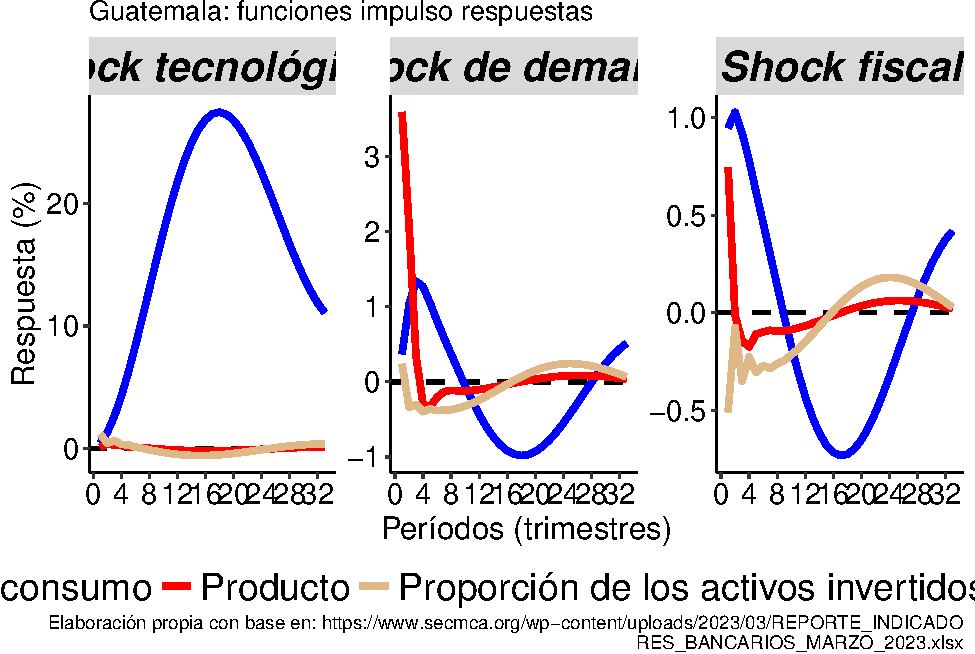
\includegraphics{01-conceptos_files/figure-latex/unnamed-chunk-4-1.pdf}

Inplicaciones

\begin{Shaded}
\begin{Highlighting}[]
\CommentTok{\#Descomposición de la varianza HISTÓRICA}
\DocumentationTok{\#\#FUNCIONES}
\NormalTok{VARhd }\OtherTok{\textless{}{-}} \ControlFlowTok{function}\NormalTok{(Estimation)\{}
  \DocumentationTok{\#\# make X and Y}
\NormalTok{  nlag    }\OtherTok{\textless{}{-}}\NormalTok{ Estimation}\SpecialCharTok{$}\NormalTok{p   }\CommentTok{\# number of lags}
\NormalTok{  DATA    }\OtherTok{\textless{}{-}}\NormalTok{ Estimation}\SpecialCharTok{$}\NormalTok{y   }\CommentTok{\# data}
\NormalTok{  QQ      }\OtherTok{\textless{}{-}} \FunctionTok{VARmakexy}\NormalTok{(DATA,nlag,}\DecValTok{1}\NormalTok{)}
  \CommentTok{\#invA   \textless{}{-} t(chol(as.matrix(summary(Estimation)$covres)))\# inverse of the A matrix}
\NormalTok{  invA    }\OtherTok{\textless{}{-}}\NormalTok{ BQMODEL}\SpecialCharTok{$}\NormalTok{LRIM}
  \CommentTok{\#invA   \textless{}{-} bqfactor}
\NormalTok{  Fcomp   }\OtherTok{\textless{}{-}} \FunctionTok{companionmatrix}\NormalTok{(Estimation)                   }\CommentTok{\# Companion matrix}
  \CommentTok{\#det    \textless{}{-} c\_case                                       \# constant and/or trends}
\NormalTok{  F1      }\OtherTok{\textless{}{-}} \FunctionTok{t}\NormalTok{(QQ}\SpecialCharTok{$}\NormalTok{Ft)                                     }\CommentTok{\# make comparable to notes}
\NormalTok{  eps     }\OtherTok{\textless{}{-}} \FunctionTok{ginv}\NormalTok{(invA) }\SpecialCharTok{\%*\%} \FunctionTok{t}\NormalTok{(}\FunctionTok{residuals}\NormalTok{(Estimation))}
  \CommentTok{\# structural errors}
\NormalTok{  nvar    }\OtherTok{\textless{}{-}}\NormalTok{ Estimation}\SpecialCharTok{$}\NormalTok{K                                 }\CommentTok{\# number of endogenous variables}
\NormalTok{  nvarXeq }\OtherTok{\textless{}{-}}\NormalTok{ nvar }\SpecialCharTok{*}\NormalTok{ nlag                                  }\CommentTok{\# number of lagged endogenous per equation}
\NormalTok{  nvar\_ex }\OtherTok{\textless{}{-}} \DecValTok{0}                                                \CommentTok{\# number of exogenous (excluding constant and trend)}
\NormalTok{  Y       }\OtherTok{\textless{}{-}}\NormalTok{ QQ}\SpecialCharTok{$}\NormalTok{Y                                             }\CommentTok{\# left{-}hand side}
  \CommentTok{\#X     \textless{}{-} QQ$X[,(1+det):(nvarXeq+det)]                    \# right{-}hand side (no exogenous)}
\NormalTok{  nobs    }\OtherTok{\textless{}{-}} \FunctionTok{nrow}\NormalTok{(Y)                                          }\CommentTok{\# number of observations}
  \DocumentationTok{\#\# Compute historical decompositions}
  \CommentTok{\# Contribution of each shock}
\NormalTok{  invA\_big    }\OtherTok{\textless{}{-}} \FunctionTok{matrix}\NormalTok{(}\DecValTok{0}\NormalTok{,nvarXeq,nvar)}
\NormalTok{  invA\_big[}\DecValTok{1}\SpecialCharTok{:}\NormalTok{nvar,] }\OtherTok{\textless{}{-}}\NormalTok{ invA}
\NormalTok{  Icomp       }\OtherTok{\textless{}{-}} \FunctionTok{cbind}\NormalTok{(}\FunctionTok{diag}\NormalTok{(nvar), }\FunctionTok{matrix}\NormalTok{(}\DecValTok{0}\NormalTok{,nvar,(nlag}\DecValTok{{-}1}\NormalTok{)}\SpecialCharTok{*}\NormalTok{nvar))}
\NormalTok{  HDshock\_big }\OtherTok{\textless{}{-}} \FunctionTok{array}\NormalTok{(}\DecValTok{0}\NormalTok{, }\AttributeTok{dim=}\FunctionTok{c}\NormalTok{(nlag}\SpecialCharTok{*}\NormalTok{nvar,nobs}\SpecialCharTok{+}\DecValTok{1}\NormalTok{,nvar))}
\NormalTok{  HDshock     }\OtherTok{\textless{}{-}} \FunctionTok{array}\NormalTok{(}\DecValTok{0}\NormalTok{, }\AttributeTok{dim=}\FunctionTok{c}\NormalTok{(nvar,(nobs}\SpecialCharTok{+}\DecValTok{1}\NormalTok{),nvar))}

  \ControlFlowTok{for}\NormalTok{ (j }\ControlFlowTok{in} \DecValTok{1}\SpecialCharTok{:}\NormalTok{nvar)\{  }\CommentTok{\# for each variable}
\NormalTok{    eps\_big }\OtherTok{\textless{}{-}} \FunctionTok{matrix}\NormalTok{(}\DecValTok{0}\NormalTok{,nvar,(nobs}\SpecialCharTok{+}\DecValTok{1}\NormalTok{)) }\CommentTok{\# matrix of shocks conformable with companion}
\NormalTok{    eps\_big[j,}\DecValTok{2}\SpecialCharTok{:}\FunctionTok{ncol}\NormalTok{(eps\_big)] }\OtherTok{\textless{}{-}}\NormalTok{ eps[j,]}
    \ControlFlowTok{for}\NormalTok{ (i }\ControlFlowTok{in} \DecValTok{2}\SpecialCharTok{:}\NormalTok{(nobs}\SpecialCharTok{+}\DecValTok{1}\NormalTok{))\{}
\NormalTok{      HDshock\_big[,i,j] }\OtherTok{\textless{}{-}}\NormalTok{ invA\_big }\SpecialCharTok{\%*\%}\NormalTok{ eps\_big[,i] }\SpecialCharTok{+}\NormalTok{ Fcomp }\SpecialCharTok{\%*\%}\NormalTok{ HDshock\_big[,(i}\DecValTok{{-}1}\NormalTok{),j]}
\NormalTok{      HDshock[,i,j] }\OtherTok{\textless{}{-}}\NormalTok{  Icomp }\SpecialCharTok{\%*\%}\NormalTok{ HDshock\_big[,i,j]}
\NormalTok{    \}}
\NormalTok{  \}}

\NormalTok{  HD.shock }\OtherTok{\textless{}{-}} \FunctionTok{array}\NormalTok{(}\DecValTok{0}\NormalTok{, }\AttributeTok{dim=}\FunctionTok{c}\NormalTok{((nobs}\SpecialCharTok{+}\NormalTok{nlag),nvar,nvar))   }\CommentTok{\# [nobs x shock x var]}

  \ControlFlowTok{for}\NormalTok{ (i }\ControlFlowTok{in} \DecValTok{1}\SpecialCharTok{:}\NormalTok{nvar)\{}
    \ControlFlowTok{for}\NormalTok{ (j }\ControlFlowTok{in} \DecValTok{1}\SpecialCharTok{:}\NormalTok{nvar)\{}
\NormalTok{      HD.shock[,j,i] }\OtherTok{\textless{}{-}} \FunctionTok{c}\NormalTok{(}\FunctionTok{rep}\NormalTok{(}\ConstantTok{NA}\NormalTok{,nlag), HDshock[i,(}\DecValTok{2}\SpecialCharTok{:}\FunctionTok{dim}\NormalTok{(HDshock)[}\DecValTok{2}\NormalTok{]),j])}
\NormalTok{    \}}
\NormalTok{  \}}

  \FunctionTok{return}\NormalTok{(HD.shock)}

\NormalTok{\}}
\DocumentationTok{\#\#\#\#\#\#\#\#\#\#}
\NormalTok{VARmakexy }\OtherTok{\textless{}{-}} \ControlFlowTok{function}\NormalTok{(DATA,lags,c\_case)\{}
\NormalTok{  nobs }\OtherTok{\textless{}{-}} \FunctionTok{nrow}\NormalTok{(DATA)}
  \CommentTok{\#Y matrix}
\NormalTok{  Y }\OtherTok{\textless{}{-}}\NormalTok{ DATA[(lags}\SpecialCharTok{+}\DecValTok{1}\NormalTok{)}\SpecialCharTok{:}\FunctionTok{nrow}\NormalTok{(DATA),]}
\NormalTok{  Y }\OtherTok{\textless{}{-}}\NormalTok{ DATA[}\SpecialCharTok{{-}}\FunctionTok{c}\NormalTok{(}\DecValTok{1}\SpecialCharTok{:}\NormalTok{lags),]}
  \CommentTok{\#X{-}matrix}
  \ControlFlowTok{if}\NormalTok{ (c\_case}\SpecialCharTok{==}\DecValTok{0}\NormalTok{)\{}
\NormalTok{    X }\OtherTok{\textless{}{-}} \ConstantTok{NA}
    \ControlFlowTok{for}\NormalTok{ (jj }\ControlFlowTok{in} \DecValTok{0}\SpecialCharTok{:}\NormalTok{(lags}\DecValTok{{-}1}\NormalTok{))\{}
\NormalTok{      X }\OtherTok{\textless{}{-}} \FunctionTok{rbind}\NormalTok{(DATA[(jj}\SpecialCharTok{+}\DecValTok{1}\NormalTok{)}\SpecialCharTok{:}\NormalTok{(nobs}\SpecialCharTok{{-}}\NormalTok{lags}\SpecialCharTok{+}\NormalTok{jj),])}
\NormalTok{    \}}
\NormalTok{  \} }\ControlFlowTok{else} \ControlFlowTok{if}\NormalTok{(c\_case}\SpecialCharTok{==}\DecValTok{1}\NormalTok{)\{ }\CommentTok{\#constant}
\NormalTok{    X }\OtherTok{\textless{}{-}} \ConstantTok{NA}
    \ControlFlowTok{for}\NormalTok{ (jj }\ControlFlowTok{in} \DecValTok{0}\SpecialCharTok{:}\NormalTok{(lags}\DecValTok{{-}1}\NormalTok{))\{}
\NormalTok{      X }\OtherTok{\textless{}{-}} \FunctionTok{rbind}\NormalTok{(DATA[(jj}\SpecialCharTok{+}\DecValTok{1}\NormalTok{)}\SpecialCharTok{:}\NormalTok{(nobs}\SpecialCharTok{{-}}\NormalTok{lags}\SpecialCharTok{+}\NormalTok{jj),])}
\NormalTok{    \}}
\NormalTok{    X }\OtherTok{\textless{}{-}} \FunctionTok{cbind}\NormalTok{(}\FunctionTok{matrix}\NormalTok{(}\DecValTok{1}\NormalTok{,(nobs}\SpecialCharTok{{-}}\NormalTok{lags),}\DecValTok{1}\NormalTok{), X)}
\NormalTok{  \} }\ControlFlowTok{else} \ControlFlowTok{if}\NormalTok{(c\_case}\SpecialCharTok{==}\DecValTok{2}\NormalTok{)\{ }\CommentTok{\# time trend and constant}
\NormalTok{    X }\OtherTok{\textless{}{-}} \ConstantTok{NA}
    \ControlFlowTok{for}\NormalTok{ (jj }\ControlFlowTok{in} \DecValTok{0}\SpecialCharTok{:}\NormalTok{(lags}\DecValTok{{-}1}\NormalTok{))\{}
\NormalTok{      X }\OtherTok{\textless{}{-}} \FunctionTok{rbind}\NormalTok{(DATA[(jj}\SpecialCharTok{+}\DecValTok{1}\NormalTok{)}\SpecialCharTok{:}\NormalTok{(nobs}\SpecialCharTok{{-}}\NormalTok{lags}\SpecialCharTok{+}\NormalTok{jj),])}
\NormalTok{    \}}
\NormalTok{    trend }\OtherTok{\textless{}{-}} \FunctionTok{c}\NormalTok{(}\DecValTok{1}\SpecialCharTok{:}\FunctionTok{nrow}\NormalTok{(X))}
\NormalTok{    X }\OtherTok{\textless{}{-}}\FunctionTok{cbind}\NormalTok{(}\FunctionTok{matrix}\NormalTok{(}\DecValTok{1}\NormalTok{,(nobs}\SpecialCharTok{{-}}\NormalTok{lags),}\DecValTok{1}\NormalTok{), }\FunctionTok{t}\NormalTok{(trend))}
\NormalTok{  \}}
\NormalTok{  A }\OtherTok{\textless{}{-}}\NormalTok{ (}\FunctionTok{t}\NormalTok{(X) }\SpecialCharTok{\%*\%} \FunctionTok{as.matrix}\NormalTok{(X))}
\NormalTok{  B }\OtherTok{\textless{}{-}}\NormalTok{ (}\FunctionTok{as.matrix}\NormalTok{(}\FunctionTok{t}\NormalTok{(X)) }\SpecialCharTok{\%*\%} \FunctionTok{as.matrix}\NormalTok{(Y))}

\NormalTok{  Ft }\OtherTok{\textless{}{-}} \FunctionTok{ginv}\NormalTok{(A) }\SpecialCharTok{\%*\%}\NormalTok{ B}
\NormalTok{  retu }\OtherTok{\textless{}{-}} \FunctionTok{list}\NormalTok{(}\AttributeTok{X=}\NormalTok{X,}\AttributeTok{Y=}\NormalTok{Y, }\AttributeTok{Ft=}\NormalTok{Ft)}
  \FunctionTok{return}\NormalTok{(retu)}
\NormalTok{\}}

\NormalTok{companionmatrix }\OtherTok{\textless{}{-}} \ControlFlowTok{function}\NormalTok{ (x)}
\NormalTok{\{}
  \ControlFlowTok{if}\NormalTok{ (}\SpecialCharTok{!}\NormalTok{(}\FunctionTok{class}\NormalTok{(x) }\SpecialCharTok{==} \StringTok{"varest"}\NormalTok{)) \{}
    \FunctionTok{stop}\NormalTok{(}\StringTok{"}\SpecialCharTok{\textbackslash{}n}\StringTok{Please provide an object of class \textquotesingle{}varest\textquotesingle{}, generated by \textquotesingle{}VAR()\textquotesingle{}.}\SpecialCharTok{\textbackslash{}n}\StringTok{"}\NormalTok{)}
\NormalTok{  \}}
\NormalTok{  K }\OtherTok{\textless{}{-}}\NormalTok{ x}\SpecialCharTok{$}\NormalTok{K}
\NormalTok{  p }\OtherTok{\textless{}{-}}\NormalTok{ x}\SpecialCharTok{$}\NormalTok{p}
\NormalTok{  A }\OtherTok{\textless{}{-}} \FunctionTok{unlist}\NormalTok{(}\FunctionTok{Acoef}\NormalTok{(x))}
\NormalTok{  companion }\OtherTok{\textless{}{-}} \FunctionTok{matrix}\NormalTok{(}\DecValTok{0}\NormalTok{, }\AttributeTok{nrow =}\NormalTok{ K }\SpecialCharTok{*}\NormalTok{ p, }\AttributeTok{ncol =}\NormalTok{ K }\SpecialCharTok{*}\NormalTok{ p)}
\NormalTok{  companion[}\DecValTok{1}\SpecialCharTok{:}\NormalTok{K, }\DecValTok{1}\SpecialCharTok{:}\NormalTok{(K }\SpecialCharTok{*}\NormalTok{ p)] }\OtherTok{\textless{}{-}}\NormalTok{ A}
  \ControlFlowTok{if}\NormalTok{ (p }\SpecialCharTok{\textgreater{}} \DecValTok{1}\NormalTok{) \{}
\NormalTok{    j }\OtherTok{\textless{}{-}} \DecValTok{0}
    \ControlFlowTok{for}\NormalTok{ (i }\ControlFlowTok{in}\NormalTok{ (K }\SpecialCharTok{+} \DecValTok{1}\NormalTok{)}\SpecialCharTok{:}\NormalTok{(K }\SpecialCharTok{*}\NormalTok{ p)) \{}
\NormalTok{      j }\OtherTok{\textless{}{-}}\NormalTok{ j }\SpecialCharTok{+} \DecValTok{1}
\NormalTok{      companion[i, j] }\OtherTok{\textless{}{-}} \DecValTok{1}
\NormalTok{    \}}
\NormalTok{  \}}
  \FunctionTok{return}\NormalTok{(companion)}
\NormalTok{\}}
\end{Highlighting}
\end{Shaded}

\begin{Shaded}
\begin{Highlighting}[]
\NormalTok{SERIE }\OtherTok{\textless{}{-}}\FunctionTok{fitted}\NormalTok{(VAR)}
\NormalTok{BQh}\OtherTok{\textless{}{-}}\FunctionTok{VARhd}\NormalTok{(VAR)}
\NormalTok{dates1}\OtherTok{\textless{}{-}} \FunctionTok{seq}\NormalTok{(}\FunctionTok{as.Date}\NormalTok{(}\StringTok{"2016{-}03{-}01"}\NormalTok{), }\AttributeTok{length=}\FunctionTok{length}\NormalTok{(SERIE[,}\DecValTok{1}\NormalTok{])}\SpecialCharTok{+}\DecValTok{2}\NormalTok{,}\AttributeTok{by=}\StringTok{"quarters"}\NormalTok{)}
\NormalTok{BQc\_T}\OtherTok{\textless{}{-}}\NormalTok{BQh[,}\DecValTok{1}\NormalTok{,}\DecValTok{1}\NormalTok{] }\CommentTok{\#SHOCK TECNOLÓGICO SOBRE c}
\NormalTok{BQc\_T}\OtherTok{\textless{}{-}}\FunctionTok{xts}\NormalTok{(BQc\_T, }\AttributeTok{order.by=}\NormalTok{dates1)}
\NormalTok{BQc\_D}\OtherTok{\textless{}{-}}\NormalTok{BQh[,}\DecValTok{1}\NormalTok{,}\DecValTok{2}\NormalTok{] }\CommentTok{\#SHOCK DEMANDA SOBRE c}
\NormalTok{BQc\_D}\OtherTok{\textless{}{-}}\FunctionTok{xts}\NormalTok{(BQc\_D, }\AttributeTok{order.by=}\NormalTok{dates1)}
\NormalTok{BQc\_F}\OtherTok{\textless{}{-}}\NormalTok{BQh[,}\DecValTok{1}\NormalTok{,}\DecValTok{3}\NormalTok{] }\CommentTok{\#SHOCK DEMANDA2 SOBRE c}
\NormalTok{BQc\_F}\OtherTok{\textless{}{-}}\FunctionTok{xts}\NormalTok{(BQc\_F, }\AttributeTok{order.by=}\NormalTok{dates1)}
\end{Highlighting}
\end{Shaded}


  \bibliography{book.bib,packages.bib}

\end{document}
